\documentclass{article}
\title{Ch. 6.1-6.2 HW}
\usepackage{graphicx, amsmath}
\graphicspath{ {./images/} }

\author{Principles of Microeconomics}
\date{\today}

\begin{document}

\maketitle

\subsection*{Quick Quiz}

\begin{enumerate}

\item (d) --

	\begin{center}
	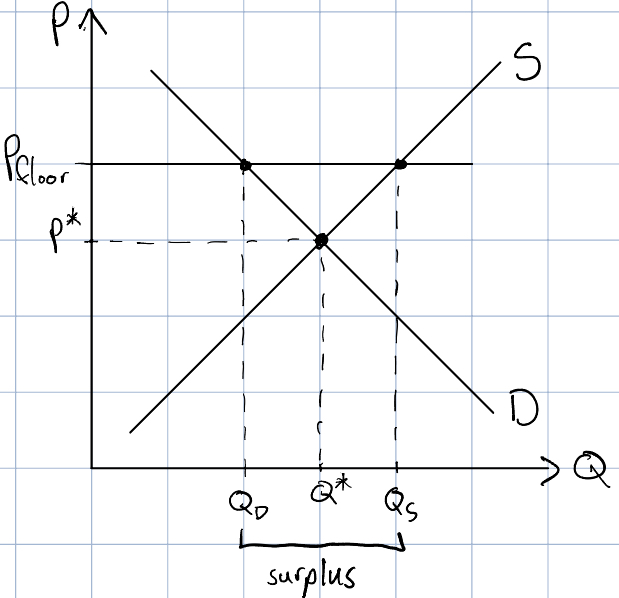
\includegraphics[width = 0.5\textwidth]{qq1}
	\end{center}
	
\item (d) --

	\begin{center}
	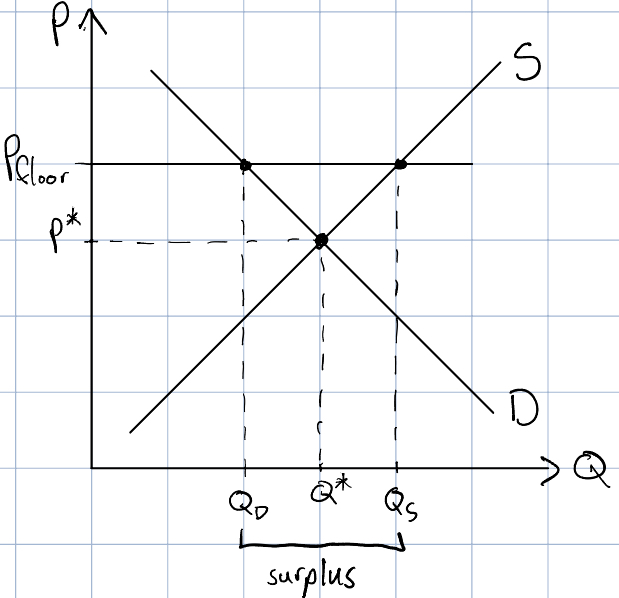
\includegraphics[width = 0.5\textwidth]{qq1}
	\end{center}
	
\item (a) -- In the long run, supply and demand for apartments become more elastic which increases the shortage.

	\begin{center}
	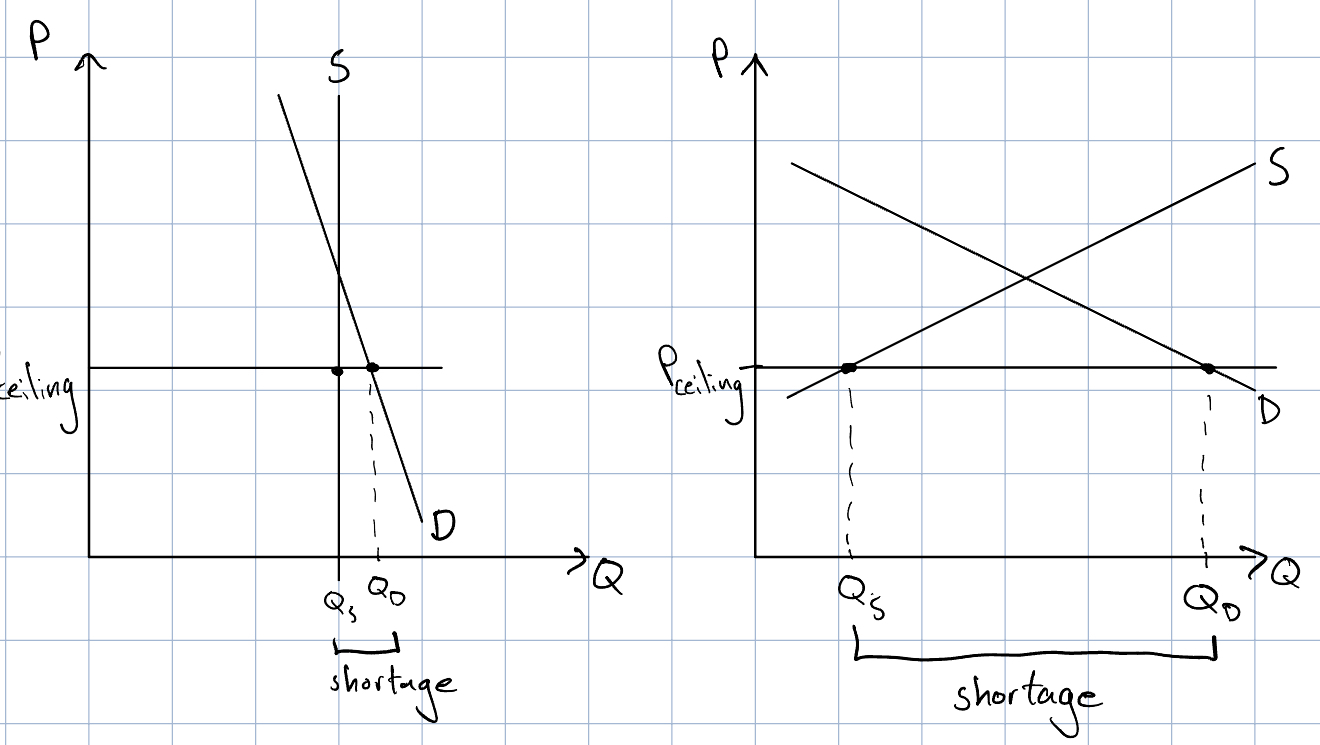
\includegraphics[width = \textwidth]{qq3}
	\end{center}

\item (c) -- Total amount paid to workers is the quantity of labor sold times the wage per unit of labor. That's the labor market analogue to revenue. If demand for labor is elastic, the increase in wage will be proportionately smaller than the decrease in quantity.

	\begin{center}
	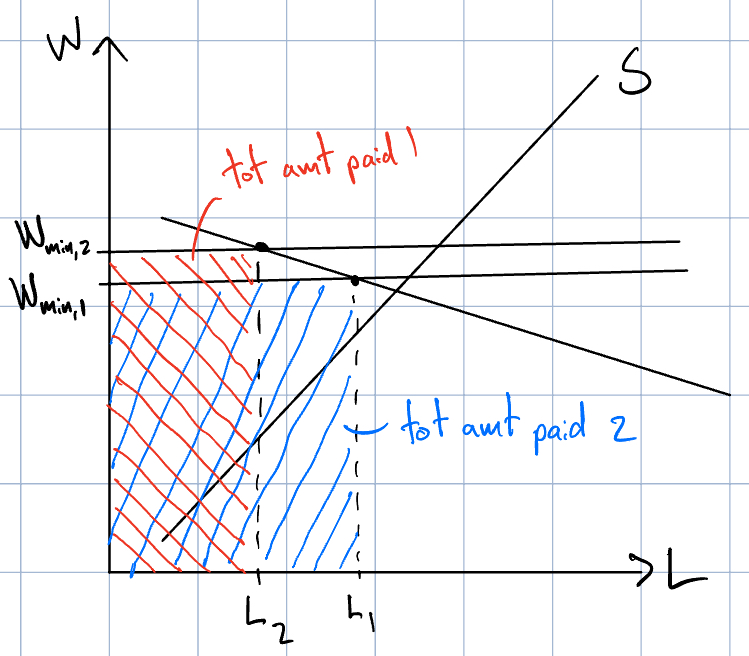
\includegraphics[width = 0.5\textwidth]{qq4}
	\end{center}
	
\end{enumerate}

\newpage

\subsection*{Problems and Applications}

\begin{enumerate}

\item If the price ceiling is non-binding, then the number of people attending comedy performances remains the same. If the price ceiling is binding, the number of people declines because the quantity of comedy performances supplied will decrease.

	\begin{center}
	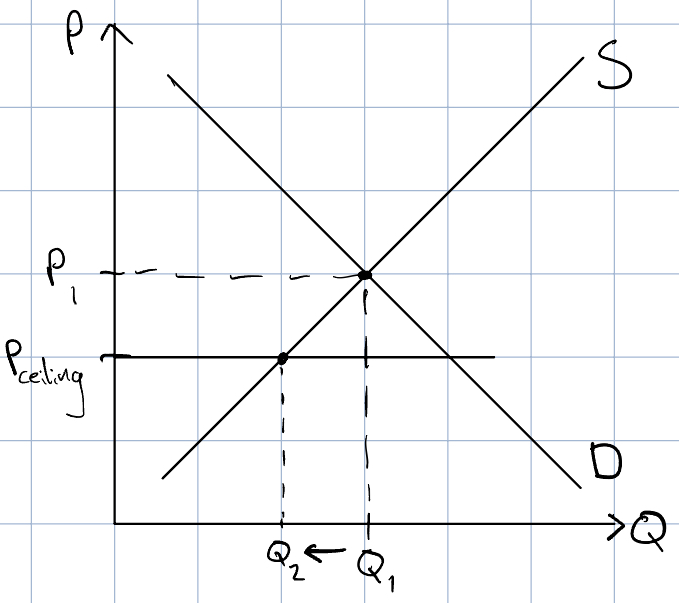
\includegraphics[width = 0.5\textwidth]{paa1}
	\end{center}
	
\item

	\begin{enumerate}
	
	\item There is a surplus. 
	
		\begin{center}
		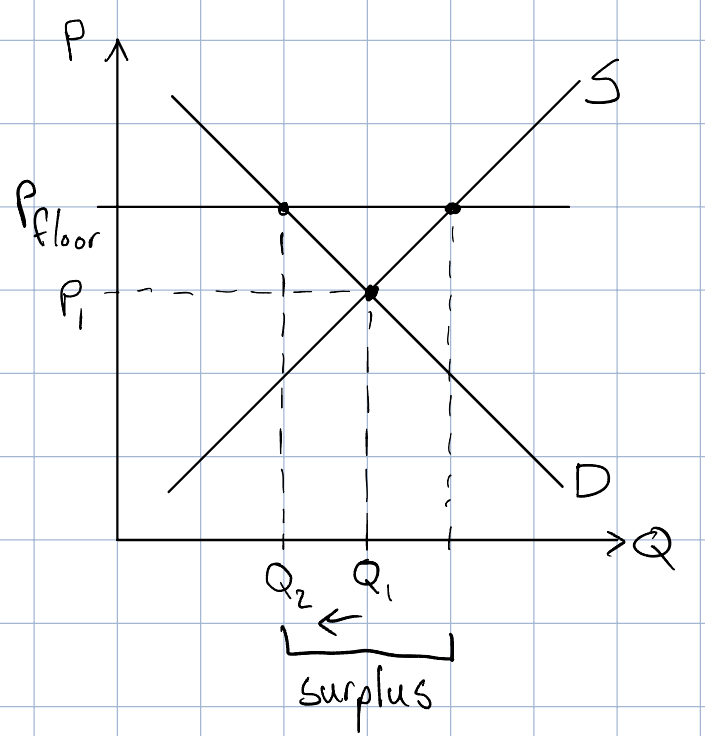
\includegraphics[width = 0.5\textwidth]{paa2a}
		\end{center}
	
	\item Yes, if demand is elastic, then the increase in price will be proportionately smaller than the decrease in quantity.
	
		\begin{center}
		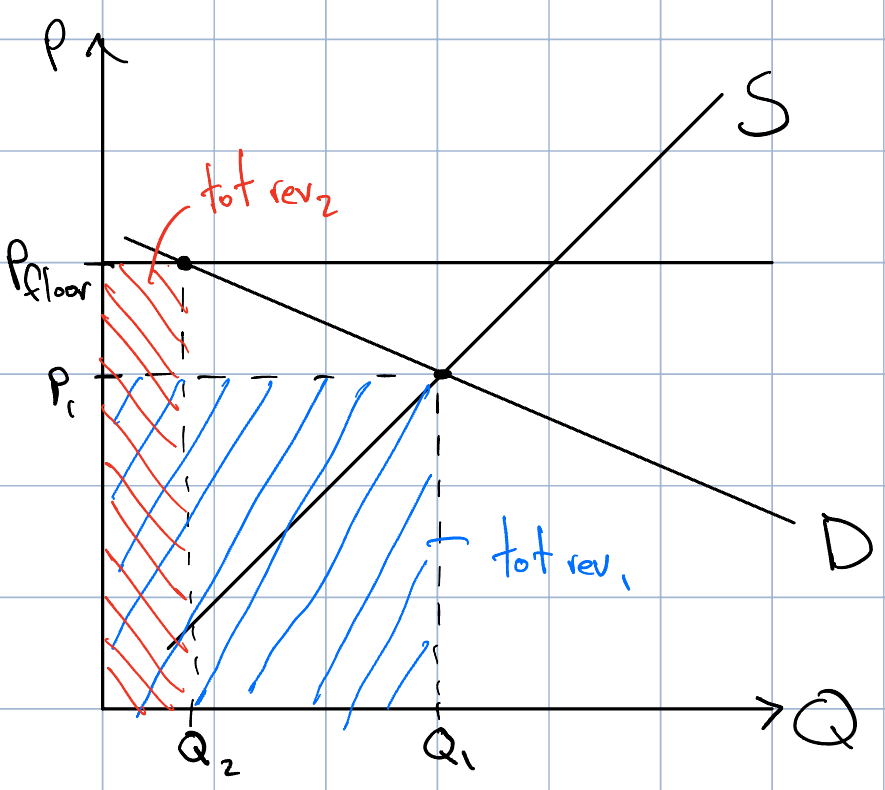
\includegraphics[width=0.5\textwidth]{paa2b}
		\end{center}
	
	\item All of the producers who couldn't find a buyer at the basic price floor benefit. Tax payers lose because the government has to spend money (raised through taxes) on cheese that buyers don't want to buy at that price.
	
	\end{enumerate}
	

\item

	\begin{enumerate}
	
	\item $(Q^*, P^*) = (6 \text{ million}, \$8)$ because $Q_S = Q_D$ when $P = \$8$.
	
	\item $P_{Floor} = \$10$. The quantity sold is the minimum of $Q_D$ and $Q_S$ because you can't force buyers to buy more than they want and you can't force sellers to sell more than they want. Since this price floor is above the equilibrium price, quantity demanded is lower than quantity supplied, and 2 million frisbees are sold.
	
	\item $P_{Ceiling} = \$9$. $P_{Ceiling} > P^*$ which means the price ceiling is non-binding. Therefore, the market moves towards equilibrium. The market price goes back to \$8, and 6 million frisbees are sold. 
	
	\end{enumerate}

\end{enumerate}

\end{document}